% \LaTeX-Main\
%% The LaTeX package incgraph - version 1.12 (2015/03/12)
%% incgraph.tex: Manual
%%
%% -------------------------------------------------------------------------------------------
%% Copyright (c) 2012-2013 by Prof. Dr. Dr. Thomas F. Sturm <thomas dot sturm at unibw dot de>
%% -------------------------------------------------------------------------------------------
%%
%% This work may be distributed and/or modified under the
%% conditions of the LaTeX Project Public License, either version 1.3
%% of this license or (at your option) any later version.
%% The latest version of this license is in
%%   http://www.latex-project.org/lppl.txt
%% and version 1.3 or later is part of all distributions of LaTeX
%% version 2005/12/01 or later.
%%
%% This work has the LPPL maintenance status `author-maintained'.
%%
%% This work consists of all files listed in README
%%
\documentclass[a4paper,11pt]{ltxdoc}

\usepackage[T1]{fontenc}
\usepackage[latin1]{inputenc}
\usepackage[english]{babel}
\usepackage{lmodern,parskip,array,ifthen,calc,makeidx}
\usepackage{amsmath,amssymb}
\usepackage[svgnames,table,hyperref]{xcolor}
\usepackage{tikz}
\usepackage[pdftex,bookmarks,raiselinks,pageanchor,hyperindex,colorlinks]{hyperref}
\urlstyle{sf}

\usepackage[a4paper,left=2.5cm,right=2.5cm,top=1.5cm,bottom=1.5cm,
    marginparsep=3mm,marginparwidth=18mm,
    headheight=0mm,headsep=0cm,
    footskip=1.5cm,includeheadfoot]{geometry}
\usepackage{fancyhdr}
\fancyhf{}
\fancyfoot[C]{\thepage}%
\renewcommand{\headrulewidth}{0pt}
\renewcommand{\footrulewidth}{0pt}
\pagestyle{fancy}
\tolerance=2000%
\setlength{\emergencystretch}{20pt}%

\RequirePackage{csquotes}
\RequirePackage[style=numeric-comp,sorting=nyt,
  maxnames=8,minnames=8,abbreviate=false,backend=biber]{biblatex}
\DeclareFieldFormat{url}{\newline\url{#1}}%
\DeclareListFormat{language}{}%
\setlength{\bibitemsep}{\smallskipamount}
\addbibresource{\jobname.bib}

\usepackage[many,listings,documentation]{tcolorbox}

\tcbset{skin=enhanced,
  doc head={colback=yellow!10!white,interior style=fill},
  doc head key={colback=magenta!5!white,interior style=fill},
  color key=DarkViolet,
  color value=Teal,
  color color=Teal,
  color counter=Orange!85!black,
  color length=Orange!85!black,
  index colorize,
  index annotate,
  %external/externalizer=tcolorbox.doc.externalizer,
}
\renewcommand*{\tcbdocnew}[1]{\textcolor{green!50!black}{\sffamily\bfseries N} #1}
\renewcommand*{\tcbdocupdated}[1]{\textcolor{blue!75!black}{\sffamily\bfseries U} #1}

\usepackage{incgraph}

\hypersetup{
  pdftitle={Manual for the incgraph package},
  pdfauthor={Thomas F. Sturm},
  pdfsubject={graphics inclusion},
  pdfkeywords={graphics inclusion page}
}

\usepackage{tikz,multicol}

\lstdefinestyle{mydocumentation}{style=tcbdocumentation,
  classoffset=0,
  texcsstyle=\color{blue},
  % LaTeX and other packages
  moretexcs={arrayrulecolor,draw,path,fill,includegraphics,ifthenelse,isodd,lipsum,path,pgfkeysalso,foreach},
  classoffset=1,
  moretexcs={%
    incgraph,incmultigraph,n,ni,nn,nt,igrset,igrpage,igrcenter,igrcenterfit,
    igrtargetset,igrboxset,igrboxcenter,igrpagestyle,igrboxtikz,igrboxtikzpage,
    igrboxtikzcenter,igrsetmatchvalue,igrsetmatches,igrifmatch,igrmakezerofill,
    },
  texcsstyle=\color{Definition}\bfseries,
  classoffset=2,
  keywordstyle=\color{Option}\bfseries,
  % option list
  morekeywords={%
    },
  classoffset=0% restore default
  }

\tcbset{documentation listing style=mydocumentation,%
  docexample/.style={enhanced,colframe=Navy!50!ExampleFrame,colback=Navy!5!ExampleBack,fontlower=\footnotesize,
    bicolor,colbacklower=ExampleBack!5!white,drop fuzzy shadow},
}

\tcbmakedocSubKey{docIgrKey}{igr}

\newcounter{texexp}

\tcbset{
  example/.code 2 args={\refstepcounter{texexp}%
  \pgfkeysalso{label={#2},docexample,listing style=mydocumentation,fonttitle=\bfseries,title={Example \thetexexp: #1}}},
}

\newenvironment{texexptitled}[3][]{%
  \hypersetup{linkcolor=white}%
  \tcbset{example={#2}{#3},listing file={\jobname.\thetexexp.listing},#1}%
  \tcblisting{}}{\endtcblisting}


\newcommand{\inputlisting}[1]{\input{\jobname.#1.listing}}
\newcommand{\inputlastlisting}{\inputlisting{\thetexexp}}

\def\version{1.12}%
\def\datum{2015/03/12}%
\makeindex


%%%%%%%%%%%%%%%%%%%%%%%%%%%%%%%%%%%%%%%%%%%%%%%%%
\begin{document}
\begin{center}
\vspace*{5mm}
\begin{tcolorbox}[enhanced,
  center upper,width=10cm,boxrule=0.4pt,
  colback=white,colframe=black!50!yellow,drop fuzzy midday shadow=black!50!yellow]
{\bfseries\LARGE The \texttt{incgraph} package\par}\medskip
{\large Manual for version \version\ (\datum)\par}
\end{tcolorbox}\bigskip
{\large Thomas F.~Sturm%
  \footnote{Prof.~Dr.~Dr.~Thomas F.~Sturm, Institut f\"{u}r Mathematik und Informatik,
    Universit\"{a}t der Bundeswehr M\"{u}nchen, D-85577 Neubiberg, Germany;
     email: \href{mailto:thomas.sturm@unibw.de}{thomas.sturm@unibw.de}} }
\end{center}
\bigskip
\begin{absquote}
  \begin{center}\bfseries Abstract\end{center}
  |incgraph| provides tools for including graphics on full paper size.
  The graphics can be centered for a given paper format or the paper may be
  resized to the graphics dimensions.
  The main use case for the package |incgraph| is to transform one or many scans
  or taken pictures to a PDF document. It can also be applied for full paper size
  \LaTeX\ created graphics.
  The package |incgraph| provides a tool box with basic macros and a
  convenience user interface which wraps the well-known |includegraphics|.
  Also, bookmarking is especially supported.
\end{absquote}

\enlargethispage*{1cm}
\tableofcontents

\begin{inctext}[paper=graphics]
  \begin{tcolorbox}[title={Caveat\hfill --- Page \thepage\ ---},
    colframe=red!65!black,colback=red!10!white,fonttitle=\Large\bfseries,
    fontupper=\large,arc=0mm,outer arc=0mm]
    This documentation contains a lot of effects which can only be seen
    when viewed on a computer screen. If you read this text on paper, you
    will not notice the paper resizing and the bookmarks. Also, pages in landscape may probably
    be rotated by your printer.
  \end{tcolorbox}
\end{inctext}


%--------------------------------------
\section{Introduction}
\subsection{Motivation}
The main purpose of this package is to include one or more graphics on full
paper size. This means that a graphic is either centered on a blank page
presumable of the given document paper size or the page is resized
to the dimensions of the graphic.
For the graphics, JPG files or PDF files or other supported formats may be
used by inclusion. Alternatively, the graphics (or whatever) can be produced
by \LaTeX\ code.
An important use case for the package |incgraph| is to transform one or many scans
or taken pictures to a PDF document. Optionally, the included graphics can
be commented with bookmarks for the resulting PDF document.

The well-known |graphicx| package \cite{carlisle:1999a} allows the inclusion
of several types of external graphics files. The convenience user interface
of |incgraph| described in Section \ref{sec:interface} relies on this package and adds
assistance for the described purpose. Note that the package is designed for and
tested with |pdflatex| to produce PDF directly. Some features like the paper
resizing may not be applicable for other work-flows.

Many of the features of the convenience user interface can be used directly
with various basic macros. These are collected and described
as a 'basic tool box' in Section \ref{sec:basictoolbox}.

If this package does not aid your intended purpose, you may take a look
at the |pdfpages| package \cite{matthias:2012a} which also supports the insertion of
external multi-page PDF documents.


\subsection{Loading the Package}
|incgraph| is loaded in the usual manner in the preamble:
\begin{dispListing}
\usepackage{incgraph}
\end{dispListing}

The package |incgraph| loads the package
|pgfkeys| \cite{tantau:2013a}. If no options are given, it also
loads the packages |pgf|, |pgffor| \cite{tantau:2013a},
the package |graphicx| \cite{carlisle:1999a}, and the
package |bookmark| \cite{oberdiek:2011a}.

\begin{itemize}
\item The option |nopgf| prevents the loading of |pgf| and |pgffor|.\\
  The opposite option |pgf| resets to loading the packages.
\item The option |nographicx| prevents the loading of |graphicx|.\\
  The opposite option |graphicx| resets to loading the package.
\item The option |nobookmark| prevents the loading of |bookmark|.\\
  The opposite option |bookmark| resets to loading the package.
\end{itemize}

So, the minimal package loading is done with the following:
\begin{dispListing}
\usepackage[nopgf,nographicx,nobookmark]{incgraph}
\end{dispListing}

Note that you can always load the mentioned packages yourself. This is
intended to avoid possible option clashes the easy way.



%--------------------------------------
\section{User Interface}\label{sec:interface}

\subsection{Inclusion Macros for External Graphics}
The macros of this section rely on the |\includegraphics| command from
the package |graphicx| \cite{carlisle:1999a}.
%Section \ref{sec:basictoolbox} describes more basic commands.

\begin{docCommand}{incgraph}{\oarg{options}\oarg{graphics options}\marg{file name}}
  The picture file with the given \meta{file name} is included in the center
  of a separate page. Depending on the \meta{options}, this page keeps the
  document size or is resized to the graphics dimensions.
  The applicable \meta{options} are listed in Section \ref{sec:keys}.
  If \meta{graphics options} are given, these are added to the options for
  the underlying |\includegraphics| command. See the documentation of
  |graphicx| \cite{carlisle:1999a} for a list of applicable \meta{graphics options}.


\begin{texexptitled}[listing only,before={\par\medskip}]%
  {The hand-drawn example (centered); see page~\pageref{exacenter}}{exacenter.listing}
\incgraph[paper=current,label={exacenter},overlay page number at bottom,
  bookmark={The hand-drawn example (centered)}]{example.jpg}
\end{texexptitled}

\begin{texexptitled}[listing only,before={\par\medskip}]%
  {The hand-drawn example (resized page); see page~\pageref{exaresized}}{exaresized.listing}
\incgraph[paper=graphics,label={exaresized},
  bookmark={The hand-drawn example (resized page)}]{example.jpg}
\end{texexptitled}

\begin{texexptitled}[listing only,before={\par\medskip}]%
  {The hand-drawn example (rotated and oversized); see page~\pageref{exarotated}}{exarotated.listing}
\incgraph[paper=current,label={exarotated},target=oversized,
  bookmark={The hand-drawn example (rotated and oversized)}]%
  [angle=30,scale=3]{example.jpg}
\end{texexptitled}
\end{docCommand}

\enlargethispage*{1cm}
\begin{docCommand}{incmultigraph}{\oarg{options}\oarg{graphics options}\marg{file name pattern}\marg{list}}
  All picture files matching the given \meta{file name pattern} where some
  parts are substituted by elements of the \meta{list}
  are included in the center of a separate page. Depending on the \meta{options}, the pages keep the
  document size or are resized to the graphics dimensions.
  The applicable \meta{options} are listed in Section \ref{sec:keys}.
  If \meta{graphics options} are given, these are added to the options for
  the underlying |\includegraphics| command. See the documentation of
  |graphicx| \cite{carlisle:1999a} for a list of applicable \meta{graphics options}.\\
  The \meta{list} may contain any construction allowed for the |\foreach| statement \cite{tantau:2013a},
  especially a list of numbers.
  The elements of the list can be used inside the \meta{file name pattern}
  with the following macros:
  \begin{itemize}
  \item\docAuxCommand{n}: The current element of the list (may be a number).
  \item\docAuxCommand{ni}: The position of the current element inside the list, i.\,e.\ |\ni|
    counts from 1 to the size of the list.
  \item\docAuxCommand{nn}: The zero-filled |\n|, if |\n| is a number. The digit
    number of |\nn| is determined by \refKey{/igr/zerofill}.
  \end{itemize}
  The resolved \meta{file name pattern} is stored inside the macro:
  \begin{itemize}
  \item\docAuxCommand{nt}: This file name may be used for bookmarking.
  \end{itemize}
  In the default behavior, non existing files are ignored.

\begin{texexptitled}[listing only,before={\par\medskip}]%
  {A series of pictures; see from page~\pageref{exaseries.1}. The image files
    exaimage-0001.png to exaimage-0150.png are included but only three
    of them exist.}{exaseries.listing}
\incmultigraph[zerofill=4,bookmark={A series of pictures: \nt},
  paper=current,label={exaseries.\n}]{exaimage-\nn.png}{1,...,150}
\end{texexptitled}
\end{docCommand}

\subsection{Inclusion Macro for Internal Graphics}

\begin{docEnvironment}{inctext}{\oarg{options}}
  The environment content is included in the center
  of a separate page. Depending on the \meta{options}, this page keeps the
  document size or is resized to the content dimensions.
  The applicable \meta{options} are listed in Section \ref{sec:keys}.


\begin{texexptitled}[listing only,before={\par\medskip}]%
  {Some text on a shrunk paper; see page~\pageref{inctext1}}{inctext1.listing}
\begin{inctext}[paper=graphics,label={inctext1},bookmark={A huge ABC}]
  \Huge ABC
\end{inctext}
\end{texexptitled}


\begin{texexptitled}[listing only,before={\par\medskip}]%
  {A tikzpicture as text content; see page~\pageref{inctext2}}{inctext2.listing}
\begin{inctext}[paper=a6,landscape,label={inctext2},bookmark={Graph},
    overlay page number at bottom=8mm]
  \begin{tikzpicture}[zustand/.style={circle,fill=Gold,draw},scale=2]
  \draw node[zustand] (s0) {$s_0$}
    +(30:3cm) node[zustand] (s1) {$s_1$}
    ++(-30:3cm) node[zustand] (s2) {$s_2$}
    +(30:3cm) node[zustand] (s3) {$s_3$};
  \path[very thick,-latex]
    (s0) edge node[above left] {a} (s1)
    edge node[below left] {b} (s2)
    (s1) edge[out=-120,in=120] node[left] {b} (s2)
    edge node[above right] {a} (s3)
    (s2) edge[out=60,in=-60] node[right] {a} (s1)
    edge node[below right] {b} (s3);
  \end{tikzpicture}
\end{inctext}
\end{texexptitled}
\end{docEnvironment}


\subsection{(Global) Option Setting}

\begin{docCommand}{igrset}{\marg{options}}
  Sets options for \refCom{incgraph}, \refCom{incmultigraph}, and
  \refEnv{inctext} inside the current \TeX\ group.
  For example, the options \refKey{/igr/paper} and
  \refKey{/igr/zerofill} may be defined for the whole document by this:
\begin{dispListing}
\igrset{paper=current,zerofill=3}
\end{dispListing}
\end{docCommand}


\clearpage
%--------------------------------------
\section{Option Keys}\label{sec:keys}

\subsection{Paper (Media) Size}\label{sec:papersize}

\begin{docIgrKey}{currentpaper}{}{no value}
  The paper size keeps unchanged at the current size
  except if \refKey{/igr/landscape} is used.
  The current paper size has not to
  be the document paper size.
  See page \pageref{exacenter} for the output
  of Example \ref{exacenter.listing} on page \pageref{exacenter.listing}.
\end{docIgrKey}

\begin{docIgrKey}{documentpaper}{}{no value}
  The paper size is set to the initial document paper size.
\end{docIgrKey}

\begin{docIgrKey}{graphicspaper}{}{no value, initially set}
  The paper is resized to the dimensions of the included image.
  The \refKey{/igr/landscape} option is ignored for this paper.
  See page \pageref{exaresized} for the output
  of Example \ref{exaresized.listing} on page \pageref{exaresized.listing}.
\end{docIgrKey}


\begin{docIgrKey}{paper size}{=\meta{width}:\meta{height}}{no default}
  The paper is resized to the given \meta{width} and \meta{height}.
\end{docIgrKey}

\begin{docIgrKey}{paper}{=\meta{name}}{no default}
  The paper size is chosen according to the given \meta{name}.
  Feasible values for the \meta{name} are
  |current|, |document|, |graphics|,
  |a0|, |a1|, |a2|, |a3|, |a4|, |a5|, |a6|, |a7|, |a8|, |a9|, |a10|,
  |b0|, |b1|, |b2|, |b3|, |b4|, |b5|, |b6|, |b7|, |b8|, |b9|, |b10|,
  |c0|, |c1|, |c2|, |c3|, |c4|, |c5|, |c6|, |c7|, |c8|, |c9|, |c10|,
  |d0|, |d1|, |d2|, |d3|, |d4|, |d5|, |d6|, |d7|,
  executive, letter, legal, ledger.
\end{docIgrKey}

\begin{docIgrKey}{landscape}{}{no value}
  If set the width and height of the chosen paper are switched. Note that
  this turns the paper by 90 degrees but the contents of the paper is not
  turned.
\end{docIgrKey}

\begin{docIgrKey}{portrait}{}{no value, initially set}
  Disables the \refKey{/igr/landscape} mode.
\end{docIgrKey}


\makeatletter%
\foreach \x in {a0,a1,a2,a3,a4,a5,a6,a7,a8,a9,a10,
  b0,b1,b2,b3,b4,b5,b6,b7,b8,b9,b10,
  c0,c1,c2,c3,c4,c5,c6,c7,c8,c9,c10,
  d0,d1,d2,d3,d4,d5,d6,d7,
  executive,letter,legal,ledger}
{\begin{docIgrKey}{\x paper}{}{no value}
  \igrset{\x paper}%
  The paper size is set to
  \texttt{\igr@target@width} $\times$ \texttt{\igr@target@height}.
\end{docIgrKey}}
\makeatother%

\begin{docIgrKey}{center}{}{no value, deprecated}
  An alias for \refKey{/igr/currentpaper}.
\end{docIgrKey}

\begin{docIgrKey}{page}{}{no value, deprecated}
  An alias for \refKey{/igr/graphicspaper}.
\end{docIgrKey}


\clearpage
\subsection{Graphics Inclusion}

\begin{docIgrKey}{options}{=\marg{graphics options}}{no default, initially empty}
  The \meta{graphics options} are applied to the underlying |\includegraphics| command.
  See the documentation of
  |graphicx| \cite{carlisle:1999a} for a list of applicable \meta{graphics options}.
\begin{texexptitled}[listing only,before={\par\medskip}]%
  {A resized image; see page~\pageref{exagraphresize}}{exagraphresize.listing}
\igrset{options={width=10cm,height=10cm}, paper=graphics,
  overlay page number at top=5mm
  }

\incgraph[bookmark={A resized image}, label={exagraphresize}]%
         {exaimage-0037.png}
\end{texexptitled}
\end{docIgrKey}

\begin{docIgrKey}{options add}{=\marg{graphics options}}{no default, initially empty}
  The \meta{graphics options} are added to the current list of options
  for the underlying |\includegraphics| command.
\end{docIgrKey}


\begin{docIgrKey}{include command}{\colOpt{=\meta{macro}}}{default and initially \cs{includegraphics}}
  Replaces the internally used \cs{includegraphics} command by the given \meta{macro}.
  Note that \meta{macro} has to have the same signature as \cs{includegraphics},
  i.\,e.\ it has to take two arguments where the first argument is optional.
\end{docIgrKey}

\begin{docIgrKey}{existence check}{=\meta{macro}}{no default}
  Replaces the internally used \cs{IfFileExists} command by the given \meta{macro}.
  Note that \meta{macro} has to have the same signature as \cs{IfFileExists},
  i.\,e.\ it has to take three arguments.
\end{docIgrKey}

\begin{docIgrKey}{fail on not found}{}{no value}
  Stops the compilation with an error if the included file does not exist.
\end{docIgrKey}

\begin{docIgrKey}{ignore on not found}{}{no value, initially set}
  Not existing included files are ignored without warning.
\end{docIgrKey}


\subsection{Hypertargets, Labels, and Bookmarks}

\begin{docIgrKey}{hyper}{}{no value, initially set}
  An automated hyper target is set to the current image. The hyper target is placed
  at the top left corner of the page. It is used internally, when a bookmark is added.
\end{docIgrKey}

\begin{docIgrKey}{no hyper}{}{no value}
  No automated hyper target is set to the current image. Use this option, if
  the package |bookmark| is not included.
\end{docIgrKey}

\begin{docIgrKey}{target}{=\meta{anchor}}{no default}
  The next hypertarget destination value is set to \meta{anchor} instead of
  an automatically created value. This may be used for hyperlinks.
\begin{dispExample}
\hyperlink{oversized}{This is linked to the oversized example (click me)}.
The target value '|oversized|' was defined in Example~\ref{exarotated.listing},
see page~\pageref{exarotated.listing}.
\end{dispExample}
\end{docIgrKey}


\clearpage

\begin{docIgrKey}{label}{=\meta{text}}{no default, initially empty}
  Adds a \LaTeX\ label to the included image.
\end{docIgrKey}


\begin{docIgrKey}{bookmark}{=\meta{text}}{no default, initially empty}
  Adds a PDF bookmark with the given \meta{text} to the current image.
\end{docIgrKey}

\begin{docIgrKey}{bookmark options}{=\marg{bookmark options}}{no default, initially empty}
  Sets the options for a bookmark.
  See the documentation of
  |bookmark| \cite{oberdiek:2011a} for a list of applicable \meta{bookmark options}.
\begin{texexptitled}[listing only,before={\par\medskip}]%
  {Bookmark options; see page~\pageref{exabookmark}}{exabookmark.listing}
% not every PDF reader will show the effect!
\igrset{bookmark options={bold,color={red}},currentpaper}
\incgraph[bookmark={This ugly image again!},label={exabookmark}]%
         {example.jpg}
\end{texexptitled}
\end{docIgrKey}

\begin{docIgrKey}{bookmark heading}{=\meta{text}}{no default, initially empty}
  For \refCom{incmultigraph}, an additional bookmark with the given \meta{text}
  is set as a heading before the images are included.
\begin{texexptitled}[listing only,before={\par\medskip}]%
  {A series of pictures; see from page~\pageref{exaheading.1}}{exaheading.listing}
\incmultigraph[zerofill=4,currentpaper,
  bookmark heading={A series of pictures},
  bookmark heading options={level=subsection},
  bookmark={\nt},bookmark options={level=subsubsection},
  overlay page number at bottom,
  label={exaheading.\n}]{exaimage-\nn.png}{1,...,150}
\end{texexptitled}
\end{docIgrKey}

\begin{docIgrKey}{bookmark heading options}{=\marg{bookmark options}}{no default, initially empty}
  Sets the options for a \refKey{/igr/bookmark heading}.
  See the documentation of
  |bookmark| \cite{oberdiek:2011a} for a list of applicable \meta{bookmark options}.
\end{docIgrKey}

\clearpage
\subsection{Borders}

The following settings enlarge or shrink the picture box, if
\refKey{/igr/graphicspaper} is used. For other paper settings, the result
will be just a certain shift of the picture box since the enlarged box
will be centered on the paper.

\begin{docIgrKey}[][doc new=2015-03-12]{left border}{=\meta{length}}{no default, initially |0pt|}
Adds a space of \meta{length} at the left hand side.
\end{docIgrKey}

\begin{docIgrKey}[][doc new=2015-03-12]{bottom border}{=\meta{length}}{no default, initially |0pt|}
Adds a space of \meta{length} at the bottom.
\end{docIgrKey}

\begin{docIgrKey}[][doc new=2015-03-12]{right border}{=\meta{length}}{no default, initially |0pt|}
Adds a space of \meta{length} at the right hand side.
\end{docIgrKey}

\begin{docIgrKey}[][doc new=2015-03-12]{top border}{=\meta{length}}{no default, initially |0pt|}
Adds a space of \meta{length} at the top.
\end{docIgrKey}

\begin{docIgrKey}[][doc new=2015-03-12]{horizontal border}{=\meta{length}}{no default, initially |0pt|}
Adds a space of \meta{length} at the left hand side and the right hand side.
\end{docIgrKey}

\begin{docIgrKey}[][doc new=2015-03-12]{vertical border}{=\meta{length}}{no default, initially |0pt|}
Adds a space of \meta{length} at the top and bottom.
\end{docIgrKey}

\begin{docIgrKey}[][doc new=2015-03-12]{border}{=\meta{length}}{no default, initially |0pt|}
Adds a space of \meta{length} at all four sides.
\end{docIgrKey}


\clearpage
\subsection{Map and Match}

\begin{docIgrKey}{set matches}{=\marg{list}}{no default, initially empty}
  The \meta{list} is a comma separated list of \meta{key}=\meta{value} pairs.
  For every pair, the given \meta{key} is mapped to the given \meta{value}.
  Later, this \meta{value} can be retrieved by
  \refKey{/igr/if match code},
  \refKey{/igr/if match set}, and
  \refKey{/igr/if match set bookmark}.

\begin{tcblisting}{docexample,listing only}
\igrset{set matches={
  foo = bar,
    1 = A very red image,
   37 = A not so centered number,
  123 = A greenish example}}
\end{tcblisting}
\end{docIgrKey}
\tcbuselistingtext

\begin{docIgrKey}{if match code}{=\marg{key}\marg{then}\marg{else}}{no default}
  If the \meta{key} was defined by \refKey{/igr/set matches},
  \refCom{igrsetmatchvalue}, or \refCom{igrsetmatches},
  the corresponding value is put in the
  macro |\igrmatchvalue| and the \meta{then} code is
  executed. If the \meta{key} is unknown, the \meta{else} code is
  executed.
\end{docIgrKey}

\begin{docIgrKey}{if match set}{=\marg{key}\marg{then}\marg{else}}{no default}
  If the \meta{key} was defined by \refKey{/igr/set matches},
  \refCom{igrsetmatchvalue}, or \refCom{igrsetmatches},
  the corresponding value is put in the
  macro |\igrmatchvalue| and |\igrset{|\meta{then}|}| is executed.
  If the \meta{key} is unknown, |\igrset{|\meta{else}|}| is executed.
\end{docIgrKey}

\begin{docIgrKey}{if match set bookmark}{=\marg{key}\marg{then}\marg{else}}{no default}
  If the \meta{key} was defined by \refKey{/igr/set matches},
  \refCom{igrsetmatchvalue}, or \refCom{igrsetmatches},
  the corresponding value is put in the
  macro |\igrmatchvalue| and the current PDF bookmark is set to \meta{then}.
  If the \meta{key} is unknown, the current PDF bookmark is set to \meta{else}.
\begin{texexptitled}[listing only,before={\par\medskip}]%
  {Map and match example; see from page~\pageref{examatch.1}}{examatch.listing}
\incmultigraph[zerofill=4,paper=graphics,
  bookmark heading={Map and match example},
  bookmark heading options={level=subsection},
  bookmark options={level=subsubsection},
  if match set bookmark={\n}{\igrmatchvalue\ (\n)}{\nt},
  overlay page number at bottom,
  label={examatch.\n}]{exaimage-\nn.png}{1,...,150}
\end{texexptitled}
\end{docIgrKey}

\begin{docIgrKey}{disable match}{}{no value, initially set}
  Disables the statements by
  \refKey{/igr/if match code},
  \refKey{/igr/if match set}, and
  \refKey{/igr/if match set bookmark}.
\end{docIgrKey}

\clearpage

\subsection{Overlays}

\begin{docIgrKey}{overlay}{=\marg{tikz code}}{no default, initially unset}
  Introduces arbitrary \meta{tikz code} to be drawn over the included image.
  Note that the |tikz| package \cite{tantau:2013a} has to be loaded separately.
  To support positioning inside the picture, two |tikz| nodes named
  |box| and |page| are defined. |box| takes the dimensions of the included image
  and |page| takes the dimensions of the image or of the page depending on the usage of
  \refKey{/igr/paper}.
\begin{texexptitled}[listing only,before={\par\medskip}]%
  {Overlay; see page~\pageref{overlay}}{overlay.listing}
\igrset{bookmark options={level=subsection}, paper=current}
\incgraph[bookmark={Picture with overlay},label={overlay},
  overlay={
    \node[draw=red,line width=3pt,fill=red,fill opacity=0.1,
          minimum width=14cm,circle] (circ) at (page.center) {};
    \node[fill=blue!5!white,below right,text width=4cm] (A)
          at ([xshift=1cm,yshift=-1cm]page.north west)
          {This included image is overlayed with |tikz| code.};
    \node[fill=green!10!white,above,text width=7cm] (B)
          at ([yshift=2cm]page.south)
          {Image Name: \nt\\Page number: \thepage\\
           Example~\ref{overlay.listing} on page~\pageref{overlay.listing}};
    \draw[line width=2pt,->] (A)--(circ);
    \draw[line width=2pt,green!50!black,dashed]
         (box.south west)--(box.south east);
    \draw[line width=2pt,->,green!50!black] (B)--(box.south);
  }]{example.jpg}
\end{texexptitled}
\end{docIgrKey}

\begin{docIgrKey}{overlay page number at}{=\meta{position}}{no default, initially unset}
  Overlays the page number at the given |tikz| \meta{position}.
\end{docIgrKey}

\begin{docIgrKey}{overlay page number at bottom}{\colOpt{=\meta{length}}}{default |1.5cm|}
  Overlays the page number at \meta{length} above the bottom edge of the paper.
  See Example~\ref{exacenter.listing} on page~\pageref{exacenter.listing}
  and the result on page~\pageref{exacenter}.
\end{docIgrKey}

\begin{docIgrKey}{overlay page number at top}{\colOpt{=\meta{length}}}{default |1.5cm|}
  Overlays the page number at \meta{length} below the top edge of the paper.
  See Example~\ref{exagraphresize.listing} on page~\pageref{exagraphresize.listing}
  and the result on page~\pageref{exagraphresize}.
\end{docIgrKey}

\begin{docIgrKey}{no overlay}{}{no value, initially set}
  Removes the overlay setting.
\end{docIgrKey}


\subsection{Miscellaneous}


\begin{docIgrKey}{pagestyle}{=\meta{page style}}{no default, initially |empty|}
  Sets the \meta{page style} for the included graphics.
\end{docIgrKey}


\begin{docIgrKey}{zerofill}{=\meta{digits}}{no default, initially |0|}
  For \refCom{incmultigraph}, the current number element
  is filled up with leading zeros until the \meta{digits} count is reached.
  If \meta{digits} is 0 or 1, nothing is added. A \meta{digits} value
  greater than 10 is treated as 10 which is the maximum number of
  possible digits. The result is accessible as |\nn|, see \refCom{incmultigraph}.
  Note that |zerofill| should be set to |0| if the list elements
  in \refCom{incmultigraph} are not numbers.
\end{docIgrKey}

\clearpage
\hypertarget{optkeyexamples}{}%
\bookmark[level=section,dest=optkeyexamples]{User Interface Examples}
\igrset{bookmark options={level=subsubsection}}
\foreach \n in {1,...,11} {\inputlisting{\n}}

\clearpage
%--------------------------------------

\section{Examples}

\subsection{Including some Scans to Standard Paper}
In this scenario, we have some scans (or images from whatever source) which
should be combined to a PDF document for our paperless office.
The paper size of the PDF document is set to a standard paper (here: letter size)
to allow the document to be printed.

The following Example \ref{somescans} is a complete template for such a document.
Here, the images |example.jpg|,
|exaimage-0001.png|,
|exaimage-0037.png|, and
|exaimage-0123.png| are used for the resulting document.
All included images are automatically bookmarked with the page number and
the file name of the source image.

\def\thecurrentexample{\jobname-example-a.tex}
\tcbinputlisting{listing file=\thecurrentexample,listing only,
  example={\texttt{\thecurrentexample}}{somescans}}

The compiled result of this stand-alone source code is not found in this document but as
a separate file in the documentation directory of the package.



\clearpage
\subsection{Creating a Picture Book}
For this example, we assume again that a bunch of image files is to be
combined to a PDF document. This time, the target document should be read or
displayed mainly on computer screens and may never be printed. Therefore,
the paper size is set flexible for the current image.

The following Example \ref{picturebook} is a complete template for such a document.
All included images are resized to a common width, but this is not necessary.
The resulting document is considered as an e-book where the bookmarks are the
most important navigation accessory.
Single page inclusions with \refCom{incgraph} are bookmarked directly, but
multi-page inclusions with \refCom{incmultigraph} can be bookmarked using the
map-and-match feature of the package.
The example shows a mixed usage of the macros.
Note that the bookmarks of the multi-page part are matched with the numbers
contained in the file names of |exaimage-0001.png| to |exaimage-0150.png|.

\def\thecurrentexample{\jobname-example-b.tex}
\tcbinputlisting{listing file=\thecurrentexample,listing only,
  example={\texttt{\thecurrentexample}}{picturebook}}

The compiled result of this stand-alone source code is not found in this document but as
a separate file in the documentation directory of the package.


\clearpage
\subsection{Reformatting from Letter to DIN A4 (and vice versa)}
In this scenario, we assume to have a PDF document with the 'wrong' paper size.
Here, |incgraph-example-a.pdf| has the letter format, but DIN A4 paper
is needed. |incgraph| is used to reformat to the desired paper size.
Of course, it also works the other way around.

The following Example \ref{reformatting} is a complete template for such a document.
The document gets the desired paper size with the \refKey{/igr/paper} option.
Then, all four pages of the original document are imported to the new paper
size. Note that the actual document content itself is not resized because
letter and DIN A4 are not so very different. If needed, the content could be
shrunk or enlarged easily by adding a |scale| option for the underlying
|\includegraphics| macro.


\def\thecurrentexample{\jobname-example-c.tex}
\tcbinputlisting{listing file=\thecurrentexample,listing only,
 example={\texttt{\thecurrentexample}}{reformatting}}

The compiled result of this stand-alone source code is not found in this document but as
a separate file in the documentation directory of the package.




\clearpage
\subsection{Drawing on Full Paper Size}



In the following examples, no external image is included to the document.
Instead, the image (or whatever) is created inside the document and put
on a separate page which could be resized or take the original document
paper size.

In Example \ref{fullpaperdrawing1}, a |tikzpicture| is drawn. The whole
picture is put inside an \refEnv{inctext} environment which puts the drawing
on a separate page which gets the dimensions of the drawing.

\begin{texexptitled}[listing only]{Creation of a special text page (resized)}{fullpaperdrawing1}
\begin{inctext}[paper=graphics, bookmark=My special text page (resized)]
\begin{tikzpicture}%
  \coordinate (A) at (0,0); \coordinate (B) at (16,16);
  \path[use as bounding box,top color=Goldenrod!25,bottom color=Navy!25]
       (A) rectangle (B);
  \coordinate (C) at ([xshift=1cm,yshift=1cm]A);
  \coordinate (D) at ([xshift=-1cm,yshift=-1cm]B);
  \path (C) -- coordinate (E) (D);
  \draw[rounded corners=5mm,very thick,Navy] (C) rectangle (D);
  \path (C) |-
    node [pos=0.75,fill=white,draw=Navy,very thick,inner sep=3mm]
      {My Special Page \thepage} (D);
  \node[text width=10cm,align=flush center,font=\Large] at (E) {
    This is my special page. It takes the dimensions of the underlying
    |tikzpicture| as seen in the source code of Example~\ref{fullpaperdrawing1}
    on page~\pageref{fullpaperdrawing1}.};
\end{tikzpicture}
\end{inctext}
\end{texexptitled}
See the result on the following page.
\clearpage\inputlastlisting


In Example \ref{fullpaperdrawing2}, nearly the same |tikzpicture| is drawn.
This time, the current paper size is used which puts the drawing
on a separate page but without resizing the paper.
To draw seamlessly, the document paper size of 21cm to 29.7cm is used
directly inside the |tikzpicture|.


\begin{texexptitled}[listing only]{Creation of a special text page (fitted)}{fullpaperdrawing2}
\begin{inctext}[paper=current, target=mytarget,
  bookmark=My special text page (fitted)]
\begin{tikzpicture}%
  \coordinate (A) at (0,0); \coordinate (B) at (21,29.7);
  \path[use as bounding box,top color=Goldenrod!25,bottom color=Navy!25]
       (A) rectangle (B);
  \coordinate (C) at ([xshift=1cm,yshift=1cm]A);
  \coordinate (D) at ([xshift=-1cm,yshift=-1cm]B);
  \path (C) -- coordinate (E) (D);
  \draw[rounded corners=5mm,very thick,Navy] (C) rectangle (D);
  \path (C) |-
    node [pos=0.75,fill=white,draw=Navy,very thick,inner sep=3mm]
      {My Special Page \thepage} (D);
  \node[text width=10cm,align=flush center,font=\Large] at (E) {
    This is my special page. It consumes the whole document paper size with
    an underlying |tikzpicture| as seen in the source code of
    Example~\ref{fullpaperdrawing2} on page~\pageref{fullpaperdrawing2}.};
\end{tikzpicture}
\end{inctext}
\end{texexptitled}


See the result on the following \hyperlink{mytarget}{page}.
\clearpage\inputlastlisting





%--------------------------------------
\section{Basic Tool Box}\label{sec:basictoolbox}
In this section, some basic macros of the package are documented.
It is assumed that most users will only need the macros from the
user interface described in Section \ref{sec:interface} and Section \ref{sec:keys}.


\subsection{Full Page Commands}

\begin{docCommand}{igrpage}{\marg{text}}
  The \meta{text} is put on a separate page which is resized to fit the
  dimensions of the \meta{text}. \meta{text} may be single letter, an
  included picture, or any \LaTeX\ code.
  The page number is stored into \docAuxCommand{theigrpage} and
  \docAuxCommand{igrAutoTarget} holds a hyper target value for bookmarking.
  The style of the separate page is set to
  the content of the macro
  \docAuxCommand{igrpagestyle} which defaults to 'empty' but can be
  redefined.
\end{docCommand}

\begin{docCommand}{igrcenter}{\marg{text}}
  The \meta{text} is put in the center of a separate page which has the
  current document dimensions. \meta{text} may be single letter, an
  included picture or any \LaTeX\ code.
  The page number is stored into \docAuxCommand{theigrpage} and
  \docAuxCommand{igrAutoTarget} holds a hyper target value for bookmarking.
  The style of the separate page is set to
  the content of the macro
  \docAuxCommand{igrpagestyle} which defaults to 'empty' but can be
  redefined.
\end{docCommand}

\begin{docCommand}{igrcenterfit}{\marg{width}\marg{height}\marg{text}}
  The \meta{text} is put in the center of a separate page which
  is resized to the given \meta{width} and \meta{height}.
  \meta{text} may be single letter, an
  included picture or any \LaTeX\ code.
  The page number is stored into \docAuxCommand{theigrpage} and
  \docAuxCommand{igrAutoTarget} holds a hyper target value for bookmarking.
  The style of the separate page is set to
  the content of the macro
  \docAuxCommand{igrpagestyle} which defaults to 'empty' but can be
  redefined.
\end{docCommand}


\begin{docCommand}{igrtargetset}{\marg{anchor}}
  The next value for \docAuxCommand{igrAutoTarget} is set to \meta{anchor}.
  This can be used for hand-made hyperlinks or bookmarks.
  An application for |igrtargetset| is found in Example~\ref{fullpaperdrawing2}
  on page~\pageref{fullpaperdrawing2}.
\end{docCommand}

\clearpage
\subsection{Box Commands}

\begin{docCommand}{igrboxset}{\marg{text}}
  The \meta{text} is put into a \TeX\ box named \docAuxCommand{igrbox}.
  Additionally, some auxiliary macros are defined:
  \begin{itemize}
  \item\docAuxCommand{igrAutoTarget}: unique value for a hyper target.
  \item\docAuxCommand{igrBoxWidth}: width of the |\igrbox|.
  \item\docAuxCommand{igrBoxHeight}: total height of the |\igrbox|.
  \item\docAuxCommand{igrBoxht}: height of the |\igrbox|.
  \item\docAuxCommand{igrBoxdp}: depth of the |\igrbox|.
  \end{itemize}
\begin{dispExample}
  \igrboxset{This is an example}
  |\igrAutoTarget| = \igrAutoTarget, |\igrBoxWidth| = \igrBoxWidth,
  |\igrBoxHeight| = \igrBoxHeight,\\
  |\igrBoxht| = \igrBoxht, |\igrBoxdp| = \igrBoxdp;
\end{dispExample}
\end{docCommand}

\begin{docCommand}{igrboxcenter}{}
  The current content of the |\igrbox|
  is put in the center of a separate page which has the
  current |pdfpage| dimensions.\\ 
  The style of the separate page is set to
  the content of the macro
  \docAuxCommand{igrpagestyle} which defaults to 'empty' but can be
  redefined.
  Note that a |\clearpage| or similar has to be inserted before this command.
\end{docCommand}

\clearpage
\begin{docCommand}{igrboxtikz}{}
  The current content of the |\igrbox| is embedded into a |\node| command
  from the |tikz| package \cite{tantau:2013a} which has to be loaded separately.
  Also, the bounding box is adjusted to the |\igrbox|.\\
  To support positioning inside the picture, two |tikz| nodes named
  |box| and |page| are defined which both take the dimensions of the |\igrbox|.
\begin{dispExample}
\igrboxset{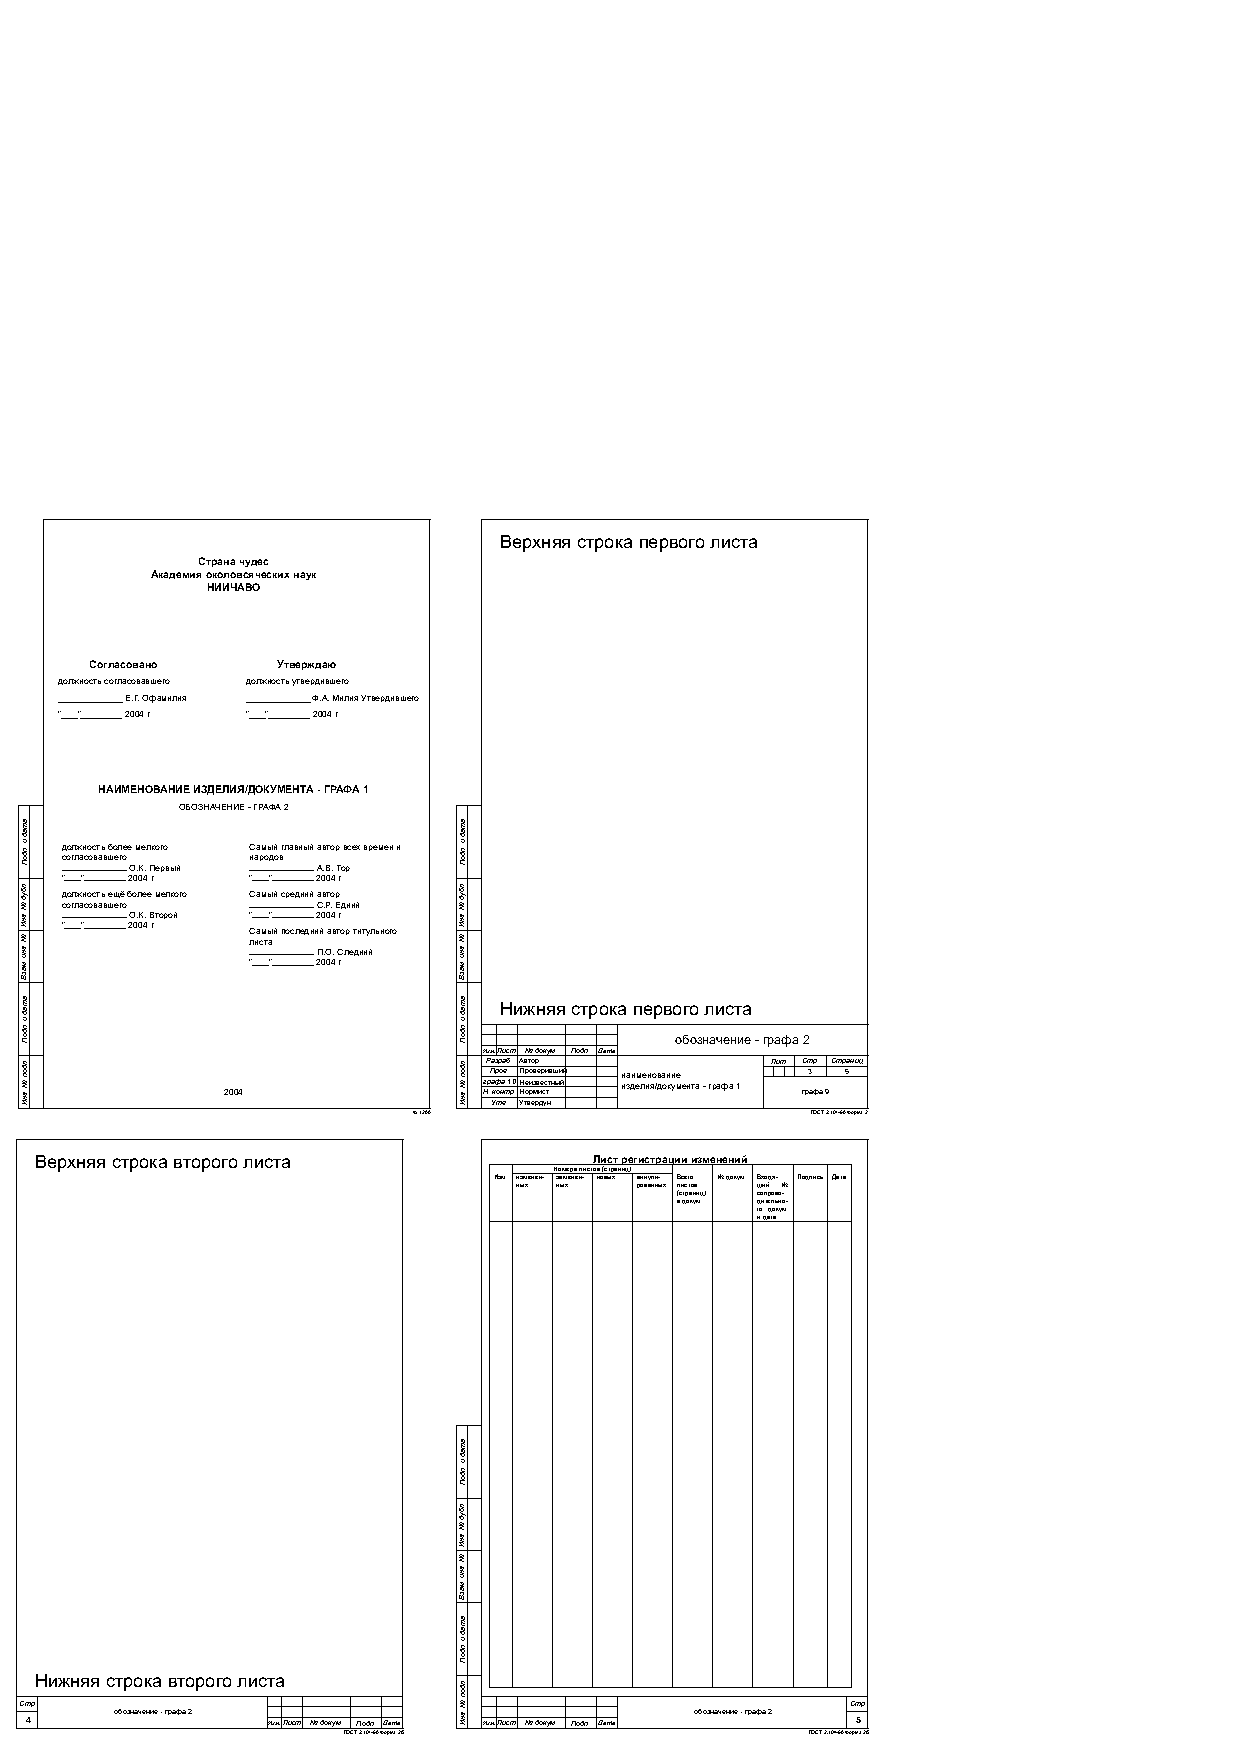
\includegraphics{example.jpg}}%
\begin{tikzpicture}%
  \igrboxtikz%
  \draw[blue,very thick] (0,0) rectangle (\igrBoxWidth,\igrBoxHeight);
  \draw[red] (0,0) grid (\igrBoxWidth,\igrBoxHeight);
  \draw[black] ([xshift=-1cm,yshift=-1cm]page.north east) circle (1cm);
\end{tikzpicture}
\end{dispExample}

The boxing macros can also be used nested (see the result on the following page):
\begin{dispListing}
\igrpage{\igrboxset{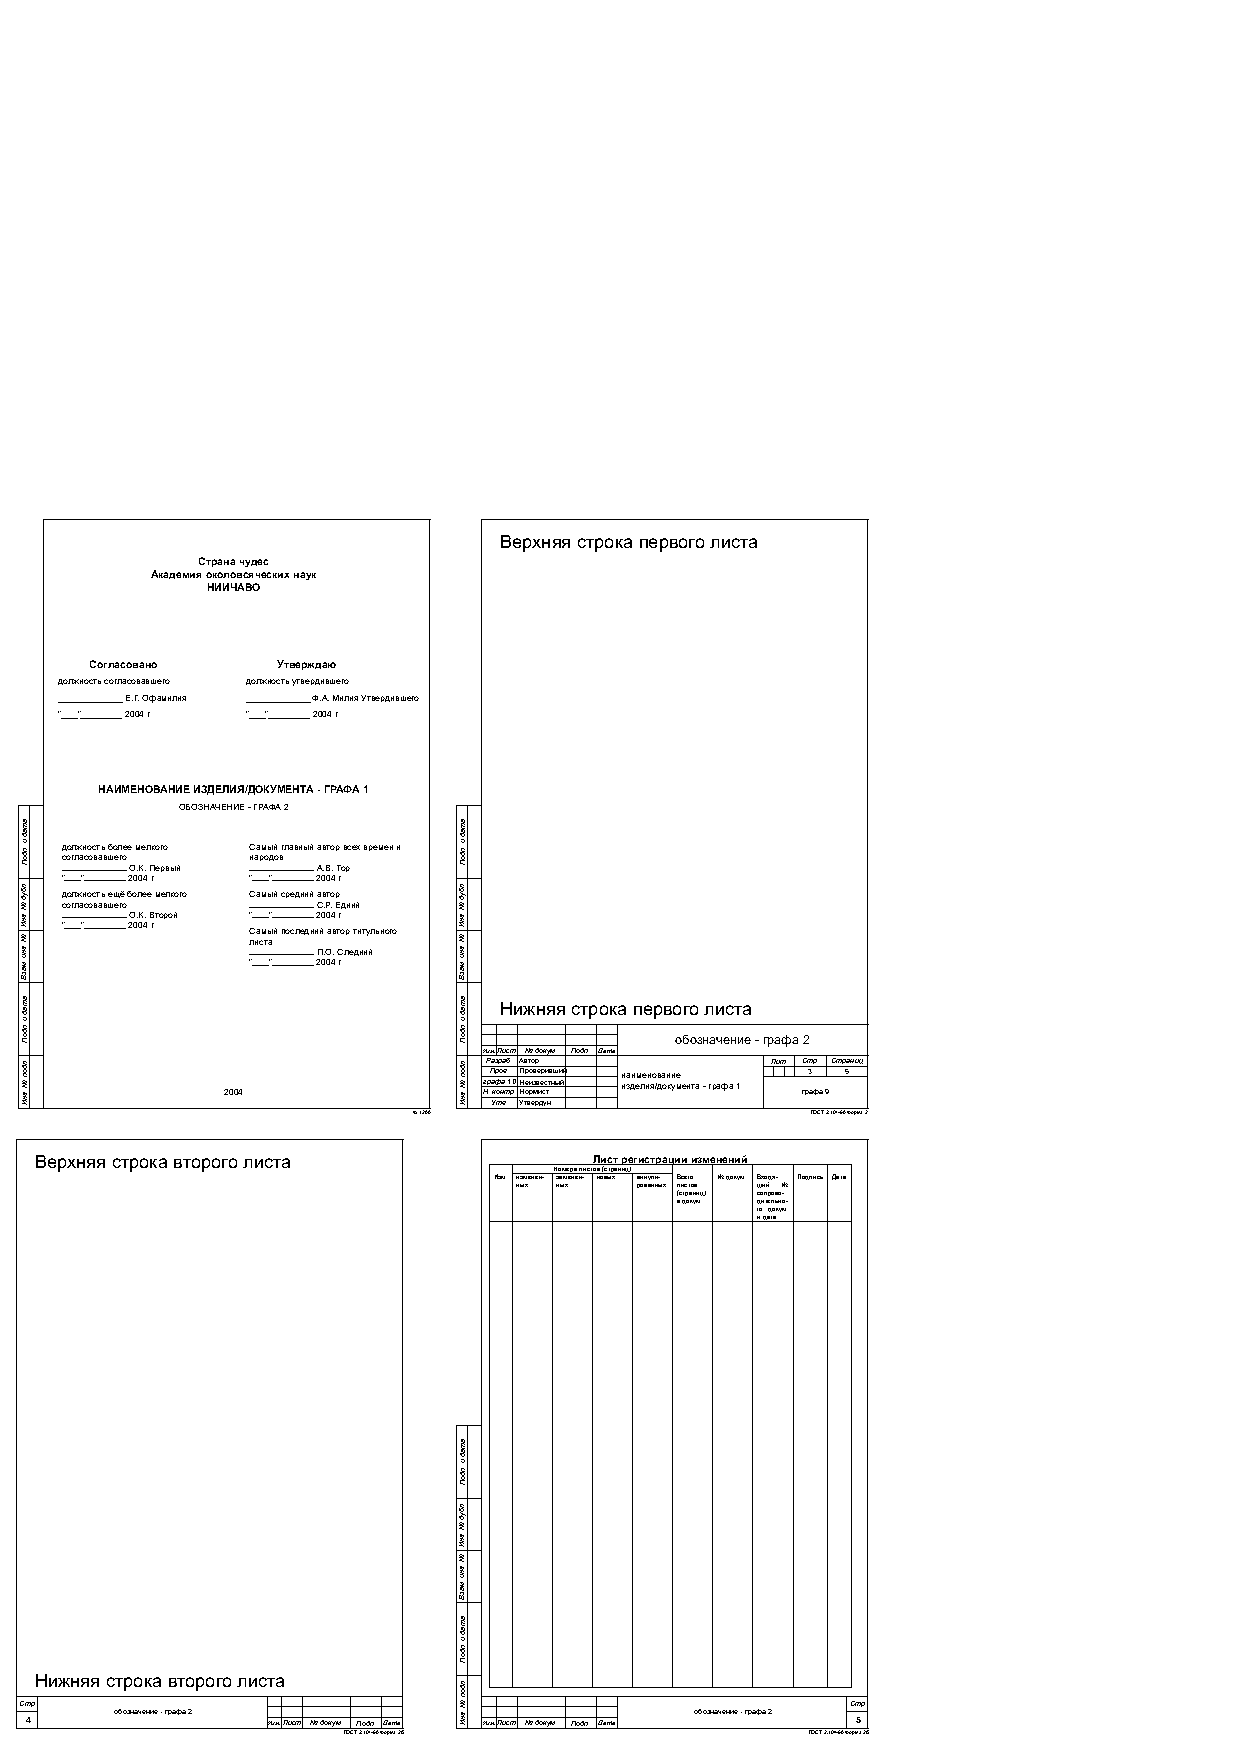
\includegraphics{example.jpg}}%
  \begin{tikzpicture}%
  \igrboxtikz%
  \draw[blue,very thick] (0,0) rectangle (\igrBoxWidth,\igrBoxHeight);
  \draw[red] (0,0) grid (\igrBoxWidth,\igrBoxHeight);
  \draw[black] ([xshift=1cm,yshift=-1cm]page.north west) circle (1cm);
\end{tikzpicture}}
\end{dispListing}
\tcbusetemp
\end{docCommand}


\begin{docCommand}{igrboxtikzpage}{}
  This is an alias for \refCom{igrboxtikz}.
\end{docCommand}


\begin{docCommand}{igrboxtikzcenter}{}
  The current content of the |\igrbox| is embedded into a |\node| command
  from the |tikz| package \cite{tantau:2013a} which has to be loaded separately.
  This node is placed in the center of a bounding box which takes the current
  page dimensions. Afterwards, |\igrBoxWidth| and |\igrBoxHeight| are
  redefined to the dimensions of the total page.\\
  To support positioning inside the picture, two |tikz| nodes named
  |box| and |page| are defined. |box| takes the dimensions of the |\igrbox|
  and |page| takes the dimensions of the |tikzpicture|.
\begin{dispListing}
\igrcenter{\igrboxset{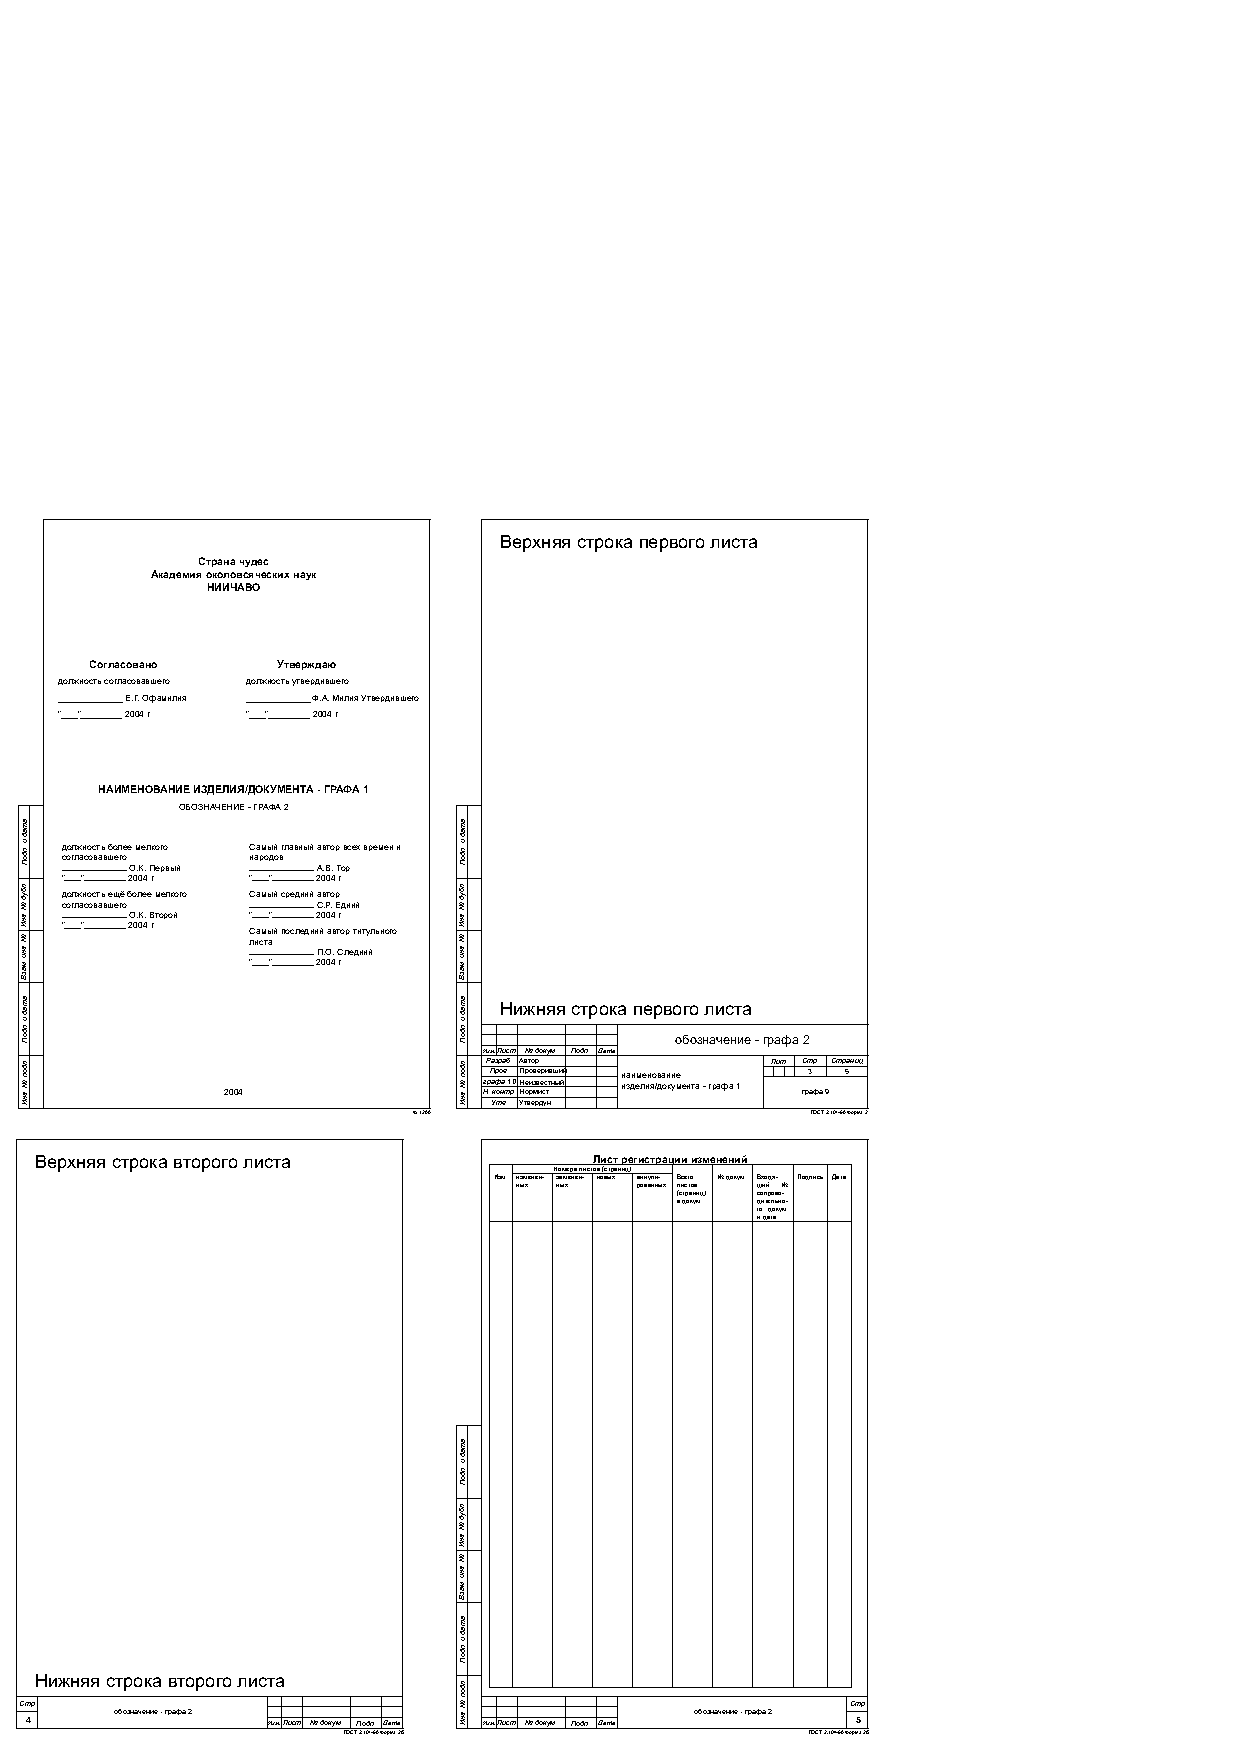
\includegraphics{example.jpg}}%
  \begin{tikzpicture}%
  \igrboxtikzcenter%
  \draw[help lines] (0,0) grid (\igrBoxWidth,\igrBoxHeight);
  \draw[dashed] (box.south west) rectangle (box.north east);

  \draw[very thick,<->] (page.north west)--(box.north west);
  \draw[very thick,<->] (page.north east)--(box.north east);
  \draw[very thick,<->] (page.south west)--(box.south west);
  \draw[very thick,<->] (page.south east)--(box.south east);
\end{tikzpicture}}
\end{dispListing}
See the result on the following page.
\tcbusetemp
\end{docCommand}


\subsection{Map and Match Commands}


\begin{docCommand}{igrsetmatchvalue}{\marg{key}\marg{value}}
  The given \meta{key} is mapped to the given \meta{value}. Later, this
  \meta{value} can be retrieved by \refCom{igrifmatch}.
\begin{dispExample}
\igrsetmatchvalue{my key A}{my value A}
\def\keytester#1{\igrifmatch{#1}{Hurray: '\igrmatchvalue'}{'#1' unknown}}

\keytester{foo}\\
\keytester{my key A}
\end{dispExample}
\end{docCommand}


\begin{docCommand}{igrsetmatches}{\marg{list}}
  The \meta{list} is a comma separated list of \meta{key}=\meta{value} pairs.
  On every pair, the \refCom{igrsetmatchvalue} macro is applied.
\begin{dispExample}
\igrsetmatches{my key A = my value A, bar = Shakespeare}
\def\keytester#1{\igrifmatch{#1}{Hurray: '\igrmatchvalue'}{'#1' unknown}}

\keytester{foo}\\
\keytester{bar}\\
\keytester{my key A}
\end{dispExample}
\end{docCommand}


\begin{docCommand}{igrifmatch}{\marg{key}\marg{then}\marg{else}}
  If a \meta{key} was defined by \refCom{igrsetmatchvalue} or
  \refCom{igrsetmatches}, the corresponding value is put in the
  macro \docAuxCommand{igrmatchvalue} and the \meta{then} code is
  executed. If the \meta{key} is unknown, the \meta{else} code is
  executed.
\begin{dispExample}
\igrsetmatches{1 = January, 2 = February, 3 = March, apr = April}
\def\monthname#1{\igrifmatch{#1}{The name of month #1\ is \igrmatchvalue.}{%
  You are kidding.}}

\monthname{1} \monthname{foo} \monthname{2}\\
\monthname{3} \monthname{apr} \monthname{35}
\end{dispExample}
\end{docCommand}


\clearpage
\subsection{Zero Filling Commands}

\begin{docCommand}{igrmakezerofill}{\marg{macro}\marg{digits}}
  With this command, a new \meta{macro} can be defined which takes a
  non negative number as parameter.
  This number is filled up with leading zeros until the
  \meta{digits} count is reached.
  If \meta{digits} is 0 or 1, nothing is added. A \meta{digits} value
  greater than 10 is treated as 10 which is the maximum number of
  possible digits.
\begin{dispExample}
\igrmakezerofill{\myfill}{0}
\myfill{7}, \myfill{12}, \myfill{934}, \myfill{665234}.\\
\igrmakezerofill{\myfill}{3}
\myfill{7}, \myfill{12}, \myfill{934}, \myfill{665234}.\\
\igrmakezerofill{\myfill}{5}
\myfill{7}, \myfill{12}, \myfill{934}, \myfill{665234}.\\
\igrmakezerofill{\myfill}{9}
\myfill{7}, \myfill{12}, \myfill{934}, \myfill{665234}.\\
\igrmakezerofill{\myfill}{30}
\myfill{7}, \myfill{12}, \myfill{934}, \myfill{665234}.
\end{dispExample}
\begin{dispExample}
\igrmakezerofill{\threedigits}{3}
\threedigits{1}%
\foreach \n in {2,...,100} {, \threedigits{\n}}.
\end{dispExample}
\end{docCommand}

\clearpage
%--------------------------------------







% Actually, it is not a good idea to include the references like this!
% Do not follow this bad example ...
\begin{tcbverbatimwrite}{\jobname.bib}

@manual{tantau:2013a,
   author    = {Till Tantau},
   title     = {The TikZ and PGF Packages},
   subtitle  = {Manual for version 3.0.0},
   url       = {http://sourceforge.net/projects/pgf/},
   date      = {2013-12-20},
}

@manual{carlisle:1999a,
   author    = {D. P. Carlisle and S. P. Q. Rahtz},
   title     = {The graphicx package},
   url       = {http://mirror.ctan.org/macros/latex/required/graphics/},
   date      = {1999-02-16},
   }

@manual{matthias:2012a,
   author    = {Andreas Matthias},
   title     = {The pdfpages Package},
   url       = {http://mirror.ctan.org/macros/latex/contrib/pdfpages/pdfpages.pdf},
   date      = {2012-04-03},
}

@manual{oberdiek:2011a,
  author    = {Heiko Oberdiek},
  title     = {The bookmark Package},
  url       = {http://mirror.ctan.org/macros/latex/contrib/oberdiek/bookmark.pdf},
  date      = {2011-12-02},
}

\end{tcbverbatimwrite}

\clearpage
\printbibliography[heading=bibintoc]

\printindex

\end{document}
